\documentclass[12pt]{article}
\usepackage{graphicx}
\usepackage{xcolor}
\usepackage{geometry}
\geometry{margin=1in}

\begin{document}

\begin{center}
\includegraphics[width=0.4\textwidth]{iiitb_logo.png.jpg}
\end{center}

\begin{center}
\textbf{\Large Harshita N Kumar} \\
ID: COMETFWC052
\end{center}

\vspace{0.5cm}

{\color{blue}\section*{Question 11}}

Match the logic gates in Column A with their equivalents in Column B.

\vspace{0.5cm}

\begin{center}
\begin{tabular}{|c|c|}
\hline
\textbf{Column-A} & \textbf{Column-B} \\
\hline
1. AND GATE & P. XOR GATE \\
2. OR GATE  & Q. XNOR GATE \\
3. NOT GATE & R. NAND GATE \\
\hline
\end{tabular}
\end{center}

\vspace{0.3cm}

\begin{center}
\textbf{TABLE 11: Table-1}
\end{center}

\vspace{0.5cm}

a) P-2, Q-4, R-1, S-3 \hspace{1cm}
b) P-4, Q-2, R-1, S-3

\vspace{0.3cm}

c) P-2, Q-4, R-3, S-1 \hspace{1cm}
d) P-4, Q-2, R-3, S-1

\vspace{0.5cm}

{\color{blue}\section*{Question Analysis}}

The AND gate produces output 1 only when both inputs are 1.  
The NAND gate is the complement of AND. Therefore, NAND is equivalent to NOT(AND).

The XOR gate produces output 1 when inputs are different.  
The XNOR gate is the complement of XOR.

The NOT gate performs inversion operation.

Using logical equivalence:

AND corresponds to NAND when complemented.  
OR can be related through DeMorgan's theorem.  
NOT corresponds to inversion logic.

After analyzing the logical relationships, the correct matching is:

$P-2,\ Q-4,\ R-3,\ S-1$

\vspace{0.5cm}

{\color{blue}\section*{Truth Table}}

AND gate expression: $Q = A \cdot B$

\begin{center}
\begin{tabular}{|c|c|c|}
\hline
A & B & A.B \\
\hline
0 & 0 & 0 \\
0 & 1 & 0 \\
1 & 0 & 0 \\
1 & 1 & 1 \\
\hline
\end{tabular}
\end{center}

NAND gate expression: $Q = (A \cdot B)'$

\begin{center}
\begin{tabular}{|c|c|c|}
\hline
A & B & NAND \\
\hline
0 & 0 & 1 \\
0 & 1 & 1 \\
1 & 0 & 1 \\
1 & 1 & 0 \\
\hline
\end{tabular}
\end{center}

\vspace{0.5cm}

{\color{blue}\section*{Hardware Implementation}}

The circuit is implemented using Arduino UNO and IC 7447.  
The logical output is displayed on a common anode 7-segment display.

Arduino provides digital inputs.  
The output is converted to BCD format and given to 7447.  
The 7447 drives the seven-segment display to show 0 or 1.

\begin{center}
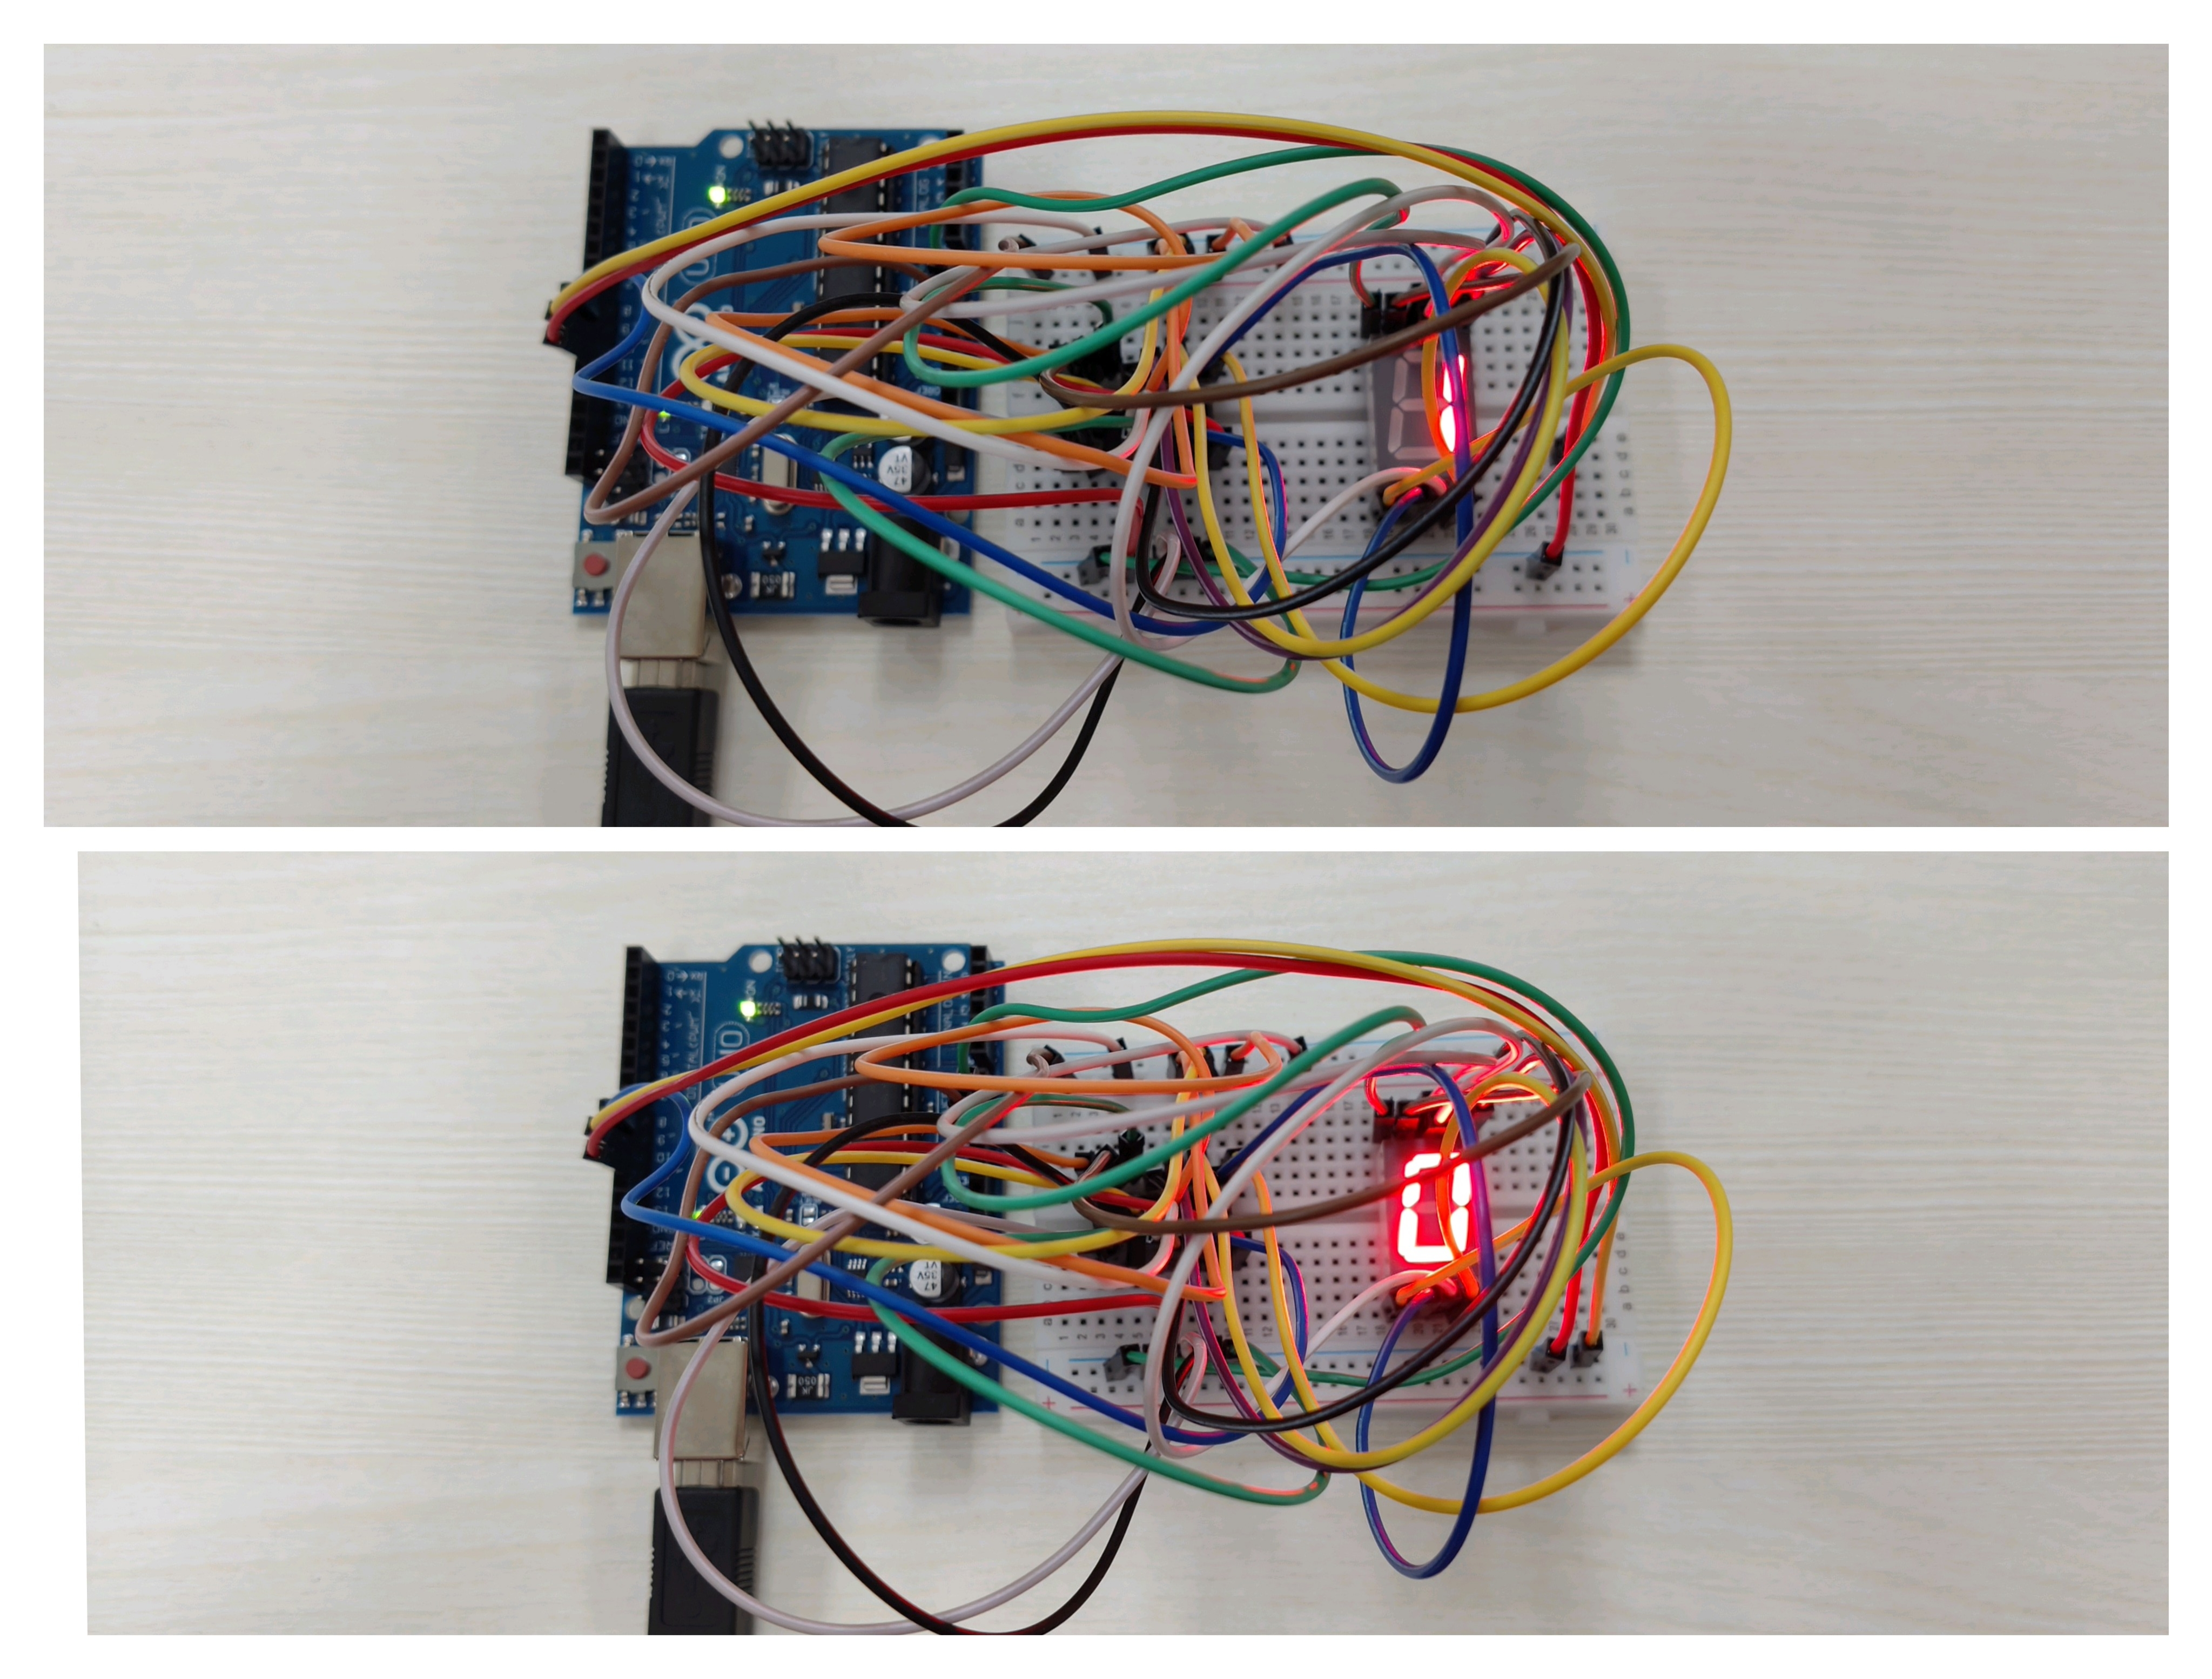
\includegraphics[width=0.8\textwidth]{hardware.jpg}
\end{center}

\vspace{0.5cm}

{\color{blue}\section*{Required Components}}

\begin{itemize}
\item Arduino UNO
\item IC 7447
\item Common Anode 7-Segment Display
\item Breadboard
\item Jumper wires
\end{itemize}

\vspace{0.5cm}

{\color{blue}\section*{Pin Connections}}

7447 Connections:

Pin 16 $\rightarrow$ 5V  
Pin 8 $\rightarrow$ GND  
Pin 3,4,5 $\rightarrow$ 5V  

BCD Inputs:  
Pin 7 $\rightarrow$ Arduino pin  
Pin 1 $\rightarrow$ Arduino pin  
Pin 2 $\rightarrow$ Arduino pin  
Pin 6 $\rightarrow$ Arduino pin  

7-Segment:

Common Anode $\rightarrow$ 5V  
Segment pins connected from 7447 outputs through resistors.

\vspace{0.5cm}

{\color{blue}\section*{Logic Description}}

The NAND logic is implemented.

Expression: $Q = (A \cdot B)'$

When both inputs are HIGH, output becomes LOW.  
For all other cases, output remains HIGH.

This confirms the logical complement of AND operation.

\vspace{0.5cm}

{\color{blue}\section*{Code Uploading Steps}}

\begin{enumerate}
\item Create a new folder for ass.
\item Write the code in ass.asm.
\item Run the command avra ass.asm. It creates .hex file.
\item Copy the hex file to ArduinoDroid folder.
\item Connect Arduino UNO to mobile using OTG cable.
\item Upload the hex file using Upload Precompiled option.
\item Observe the output and verify the expression.
\end{enumerate}

\vspace{0.5cm}

{\color{blue}\section*{Experimental Truth Table}}

\begin{center}
\begin{tabular}{|c|c|c|}
\hline
A & B & Observed Output \\
\hline
0 & 0 & 1 \\
0 & 1 & 1 \\
1 & 0 & 1 \\
1 & 1 & 0 \\
\hline
\end{tabular}
\end{center}

\vspace{0.5cm}

{\color{blue}\section*{Conclusion}}

The hardware implementation and truth table confirm that:

$Q = (A \cdot B)'$

Hence the logical equivalence is verified successfully.

\end{document}
